% !TeX program = xelatex
\documentclass[12pt,a4paper]{article}
\usepackage{fontspec}
\setmainfont{Times New Roman}
\usepackage[english,russian]{babel}
\usepackage{amsmath,amssymb,mathrsfs,cancel}
\usepackage[margin=22mm]{geometry}
\usepackage{graphicx,float}
\usepackage[unicode,hidelinks]{hyperref}
\DeclareMathOperator{\grad}{grad}
\DeclareMathOperator{\Div}{div}
\newcommand{\Rey}{\mathrm{Re}}
\setlength{\emergencystretch}{3em}
\sloppy
\interfootnotelinepenalty=10000
\newcommand{\topic}[1]{\par\medskip\noindent\textbf{#1}\par\nobreak\smallskip}
\renewcommand{\thefootnote}{\arabic{footnote})}
\begin{document}
\section*{Вопрос 10}
Описание многофазной фильтрации. Обобщенный закон Дарси, относительная фазовая проницаемость. Учет капиллярной разности давлений между фазами, функция Леверетта.

\medskip
\noindent\textbf{Источник:} К. С. Басниев, А. М. Власов, И. Н. Кочина, В. М. Максимов. \textit{Подземная гидравлика}. Москва: Недра, 1986. Глава 1, § 5, с. 19--22; глава 9, §§ 2--3, с. 199--204.
\par\bigskip
\section*{Глава 1. Основные понятия и законы фильтрации нефти, газа и воды}
\subsection*{§ 5. Обобщенный закон Дарси}
% Источник: Basniev-et-al.djvu; печатная страница: 19; страница файла: 20
Закон Дарси для течения в пористой среде однородной жидкости можно распространить на случай совместного течения двух несмешивающихся жидкостей, обобщив понятие проницаемости.

Прежде всего введем понятие скорости фильтрации данной фазы $\vec w_i$. Аналогично скорости фильтрации однородной жидкости $\vec w_i$ определяется как вектор, проекция которого на некоторое направление $l$ равна отношению объемного расхода данной фазы к площадке $\Omega_l$, перпендикулярной к указанному направлению:
\begin{equation}(\vec w_i)_l=Q_i/\Omega_l.\tag{1.15}\label{q10:eq-1-15}\end{equation}
Площадка $\Omega_l$ пересекает твердую и обе подвижные фазы.

При фильтрации двух несмешивающихся жидкостей вводят понятие насыщенности порового пространства фазой. Насыщенность элемента пористой среды данной фазой $\sigma_i$ определяется как относительная часть объема активных пор среды, занятая этой фазой:
\begin{equation}\sigma_i=\Delta V_i/\Delta V_\text{п},\tag{1.16}\label{q10:eq-1-16}\end{equation}
где $i$ принимает значения 1 и 2 ($\sigma_1,\sigma_2$ --- насыщенность соответственно смачивающей и несмачивающей фазами).

Здесь $\Delta V_i$ --- объем среды, занятой жидкостью $i$; $\Delta V_\text{п}$ --- общий объем активных пор в данном элементе. Очевидно, справедливо равенство
\begin{equation}\sigma_1+\sigma_2=1,\tag{1.17}\label{q10:eq-1-17}\end{equation}
поэтому из двух насыщенностей только одна независима и обычно характеристики движения в потоке двухфазной жидкости представляются в функции от насыщенности первой (смачивающей) фазой и вводится обозначение $\sigma=\sigma_1$.

Экспериментально установлено, что расход каждой фазы растет с увеличением перепада давления и насыщенности данной фазой, а закон фильтрации каждой из фаз по аналогии с законом Дарси можно записать в виде
\begin{equation}w_1=\frac{k_1^*\Delta p_1}{\mu_1L},\qquad w_2=\frac{k_2^*\Delta p_2}{\mu_2L},\tag{1.18}\label{q10:eq-1-18}\end{equation}
где $w_1$ и $w_2$ --- скорости фильтрации фаз; $\mu_1$ и $\mu_2$ --- динамические коэффициенты вязкости жидкостей; $\Delta p_1$ и $\Delta p_2$ --- разности давлений в соответствующих фазах; $k_1^*$ и $k_2^*$ --- фазовые проницаемости. Величины $k_i^*$ ($i=1,2$) являются для $i$-й жидкости проницаемостями в обычном смысле в условиях совместной фильтрации. Эти величины зависят от природы пористой среды (и, прежде всего, от ее абсолютной проницаемости $k$, определяемой по данным о фильтрации однородной жидкости), а также от насыщенности пористой среды каждой фазой. При описании двухфазных течений обычно вместо фазовых проницаемостей $k_i^*$ вводят так называемые
% Источник: Basniev-et-al.djvu; печатная страница: 20; страница файла: 21
«относительные проницаемости» $k_i$ фаз, определяемые из отношений
\begin{equation}k_1=k_1^*/k,\qquad k_2=k_2^*/k.\tag{1.19}\label{q10:eq-1-19}\end{equation}
В большинстве опытов показано, что для данной структуры пористой среды относительные проницаемости $k_i$ являются в основном функциями насыщенности, а если и наблюдается влияние иных параметров (например, отношения коэффициентов вязкости $\mu_0$ фаз), то им обычно пренебрегают. Тогда с учетом \eqref{q10:eq-1-19} закон Дарси \eqref{q10:eq-1-18} для каждой из фаз записывается в виде
\begin{equation}w_i=k\frac{k_i(\sigma)\Delta p_i}{\mu_iL},\qquad i=1,2.\tag{1.20}\label{q10:eq-1-20}\end{equation}
В общем случае давления $p_1$ и $p_2$ в фазах не будут совпадать из-за действия поверхностного натяжения и связаны равенством
\begin{equation}p_2-p_1=p_\text{к},\tag{1.21}\label{q10:eq-1-21}\end{equation}
где $p_\text{к}$ --- капиллярное давление.
\renewcommand{\thefigure}{1.\arabic{figure}}\setcounter{figure}{5}
\begin{figure}[H]\centering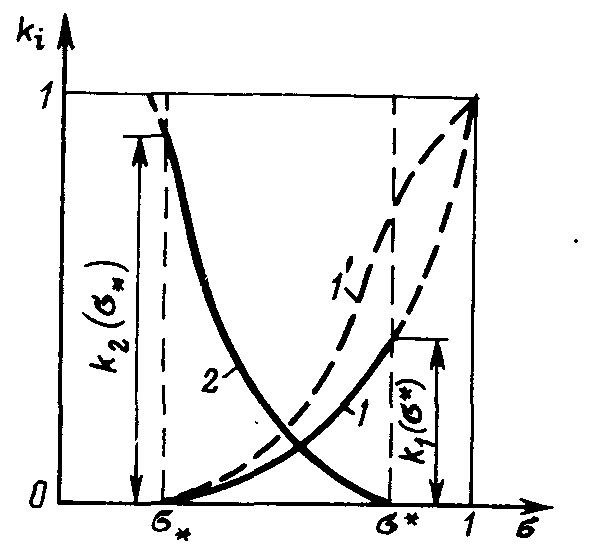
\includegraphics[width=.55\linewidth]{figures/fig-1-6.png}\caption{Кривые зависимости относительных проницаемостей от насыщенности}\label{q10:fig-1-6}\end{figure}
Типичный вид экспериментальных кривых фазовых проницаемостей $k_i(\sigma)$ приведен на рис. \ref{q10:fig-1-6} (кривая \textit{1} относится к более смачивающей жидкости --- воде, кривая \textit{2} --- к менее смачивающей --- нефти; кривая $1'$ относится к случаю, когда первая фаза является газом и $\sigma$ --- газонасыщенность). Отметим некоторые характерные особенности этих кривых. Для каждой фазы существует предельная насыщенность ($\sigma_*$ и $1-\sigma^*$) такая, что при меньших значениях насыщенности эта фаза неподвижна. Движение первой фазы может происходить только в том случае, если $\sigma>\sigma_*$ (для водонефтяной системы $\sigma_*$ называют насыщенностью связанной водой). Для второй фазы связанная насыщенность равна $1-\sigma^*$ и называется остаточной нефтенасыщенностью. Таким образом, совместное течение двух фаз имеет место лишь в следующем интервале изменения насыщенности жидкостью 1:
\[\sigma_*\le\sigma\le\sigma^*.\]
Сумма относительных проницаемостей для каждого фиксированного значения $\sigma$ меньше 1:
\[k_1(\sigma)+k_2(\sigma)<1,\qquad0<\sigma<1.\]
Графики $k_i(\sigma)$ представляют собой асимметричные кривые (см. рис. \ref{q10:fig-1-6}). Относительная проницаемость $k_1(\sigma)$ смачивающей фазы при $\sigma=\sigma^*$ имеет значение, меньшее 1, тогда как величина $k_2(\sigma)$ при $\sigma=\sigma_*$ близка к единице. Это означает, что присутствие связанной смачивающей фазы мало влияет на течение несмачивающей
% Источник: Basniev-et-al.djvu; печатная страница: 21; страница файла: 22
жидкости, тогда как присутствие остаточной несмачивающей фазы значительно «стесняет» движение смачивающей фазы.

Заметим, что, как показывают опыты и анализ размерностей, относительные проницаемости $k_i(\sigma)$ не зависят от размеров пор, но могут зависеть от их формы и распределения. Поэтому кривые одинаковы для определенных групп, сходных по структуре пористых сред.

Приведем здесь приближенные эмпирические формулы, которыми можно пользоваться при оценочных расчетах.

1. Для воды и нефти ($\sigma$ --- водонасыщенность)
\[\begin{aligned}
k_1(\sigma)&=\begin{cases}0&\text{при }0\le\sigma\le0{,}2,\\{}[(\sigma-0{,}2)/0{,}8]^{3{,}5}&\text{при }0{,}2\le\sigma\le1;\end{cases}\\
k_2(\sigma)&=\begin{cases}[(0{,}85-\sigma)/0{,}85]^{2{,}8}(1+2{,}4\sigma)&\text{при }0\le\sigma\le0{,}85,\\0&\text{при }0{,}85\le\sigma\le1.\end{cases}
\end{aligned}\]
\begin{figure}[H]\centering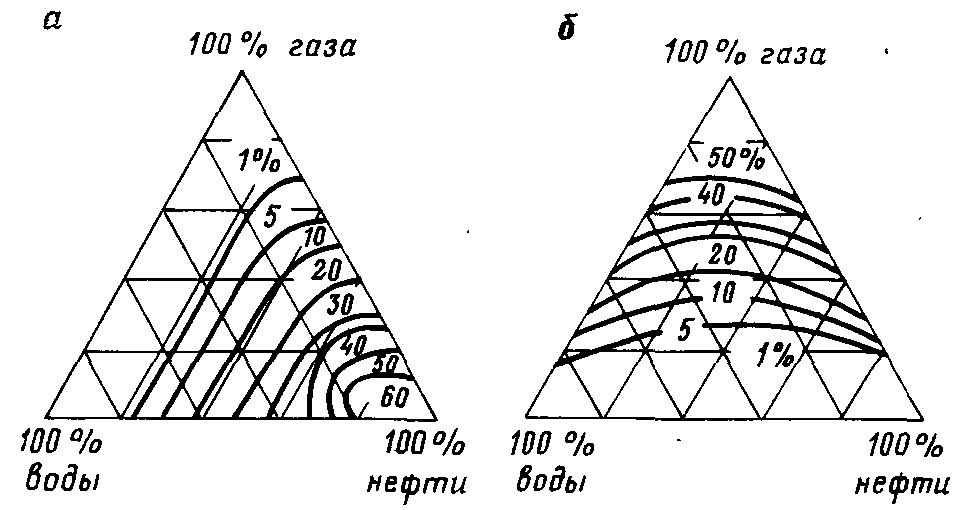
\includegraphics[width=.8\linewidth]{figures/fig-1-7.png}\caption{Диаграммы фазовых проницаемостей для трехфазной смеси (вода---нефть---газ): \textit{а} --- для нефти; \textit{б} --- для газа}\label{q10:fig-1-7}\end{figure}
2. Для газа и воды ($\sigma$ --- газонасыщенность)
\[\begin{aligned}
k_1(\sigma)&=\begin{cases}0&\text{при }0\le\sigma\le0{,}1,\\{}[(\sigma-0{,}1)/0{,}9]^{3{,}5}(4-3\sigma)&\text{при }0{,}1\le\sigma\le1;\end{cases}\\
k_2(\sigma)&=\begin{cases}[(0{,}8-\sigma)/0{,}8]^{3{,}5}&\text{при }0\le\sigma\le0{,}8,\\0&\text{при }0{,}8\le\sigma\le1.\end{cases}
\end{aligned}\]
Введенные выше понятия можно обобщить на случай совместного движения трех несмешивающихся флюидов: нефти, газа и воды. Если обозначить эти жидкости соответственно индексами «н», «г» и «в», то можно ввести относительные проницаемости $k_\text{н}$, $k_\text{г}$ и $k_\text{в}$ точно так же, как это было сделано для двух жидкостей. При этом фазовые проницаемости являются уже функциями двух независимых насыщенностей $\sigma_\text{н}$ и $\sigma_\text{в}$ (газонасыщенность $\sigma_\text{г}=1-\sigma_\text{н}-\sigma_\text{в}$):
\begin{equation}k_\text{н}=k_\text{н}(\sigma_\text{н},\sigma_\text{в}),\quad k_\text{в}=k_\text{в}(\sigma_\text{н},\sigma_\text{в}),\quad k_\text{г}=k_\text{г}(\sigma_\text{н},\sigma_\text{в}),\tag{1.22}\label{q10:eq-1-22}\end{equation}
и определяются с помощью треугольных диаграмм (рис. \ref{q10:fig-1-7}, \textit{а} ---
% Источник: Basniev-et-al.djvu; печатная страница: 22; страница файла: 23
для нефти $k_\text{н}$ и рис. \ref{q10:fig-1-7}, \textit{б} --- для газа $k_\text{г}$). Принцип построения этих диаграмм следующий. Параллельно каждой стороне треугольника проводятся прямые, вдоль которых насыщенность одной из фаз постоянна. Каждая насыщенность изменяется от нуля вдоль стороны треугольника до 100\% на противолежащей вершине. Каждая точка внутри треугольника, находящаяся на пересечении двух прямых, параллельных двум сторонам, соответствует определенным значениям $\sigma_\text{н}$, $\sigma_\text{в}$ и $\sigma_\text{г}=1-\sigma_\text{н}-\sigma_\text{в}$. На треугольники наносятся линии одинаковых относительных проницаемостей фаз. На рис. \ref{q10:fig-1-7}, \textit{а} проведены линии равных значений относительной проницаемости для нефти $k_\text{н}$, на рис. \ref{q10:fig-1-7}, \textit{б} --- для газа $k_\text{г}$.

Характер зависимостей \eqref{q10:eq-1-22} определяется различной степенью смачивания твердых зерен породы фазами, причем оказывается, что относительная проницаемость наиболее смачивающей фазы --- воды практически зависит только от водонасыщенности $\sigma_\text{в}$ и почти не зависит от нефте- и газонасыщенности $\sigma_\text{н}$ и $\sigma_\text{г}$.

\section*{Глава 9. Основы теории фильтрации многофазных систем}
\subsection*{§ 2. Основные характеристики многофазной фильтрации}
% Источник: Basniev-et-al.djvu; печатная страница: 199; страница файла: 200
Углеводородные системы могут быть гомо- и гетерогенными. В гомогенной системе все ее части имеют одинаковые физические и химические свойства. Составляющие гомогенной системы (называемые компонентами) «размазаны» по всему пространству и взаимодействуют на молекулярном уровне. Для гетерогенной системы физические и химические свойства в разных точках различны. Гетерогенные системы состоят из фаз. Фаза --- это часть системы, которая является гомогенной и отделена от других фаз отчетливыми границами. Смесь воды, нефти и газа в пласте --- типичный пример гетерогенной среды.

Главными характеристиками движения многофазной системы являются насыщенность и скорость фильтрации каждой фазы.

Насыщенностью $\sigma_i$ порового пространства $i$-й фазой называется доля объема пор $\Delta V_i$, занятая этой фазой в элементарном объеме:
\begin{equation}\sigma_i=\Delta V_i/\Delta V_\text{п},\quad i=1,2,\ldots,n.\tag{9.1}\label{q10:eq-9-1}\end{equation}
Очевидно, что
\begin{equation}\sum_{i=1}^n\sigma_i=1.\tag{9.2}\label{q10:eq-9-2}\end{equation}
% Источник: Basniev-et-al.djvu; печатная страница: 200; страница файла: 201
Таким образом, в $n$-фазной системе имеется $(n-1)$ независимая насыщенность. В частности, при исследовании фильтрации смеси двух фаз используется лишь одна из насыщенностей, которая обозначается в дальнейшем $\sigma$ (обычно это насыщенность вытесняющей фазы).

Движение каждой из фаз характеризуется вектором скорости фильтрации $\vec w_i$ данной фазы, который (по аналогии со скоростью фильтрации однородной жидкости) определяется как вектор, проекция которого на некоторое направление $l$ равна отношению объемного расхода $Q_i$ данной фазы к площадке $\Omega_l$, перпендикулярной к указанному направлению:
\begin{equation}(\vec w_i)_l=Q_i/\Omega_l,\quad i=1,2,\ldots,n.\tag{9.3}\label{q10:eq-9-3}\end{equation}
Площадка $\Omega_l$ пересекает как твердую, так и подвижные фазы.

При изучении сложных фильтрационных процессов возникает необходимость в построении моделей многофазных (гетерогенных) систем, в которых каждая фаза, в свою очередь, моделируется многокомпонентной гомогенной смесью. При этом между компонентами возможны химические реакции, переход компонентов из одной фазы в другую, процессы адсорбции, диффузии и др. В дальнейшем для простоты и лучшего понимания физической сути происходящих процессов ограничимся рассмотрением двухфазной фильтрации (например, нефти и воды или воды и газа).

При совместном течении двух фаз в пористой среде, по крайней мере, одна из них образует систему, граничащую со скелетом породы и частично с другой жидкостью. Из-за избирательного смачивания твердой породы одной из жидкостей площадь контакта каждой из фаз со скелетом пористой среды значительно превышает площадь контакта фаз между собой. Это позволяет предположить, что каждая фаза движется по занятым ею поровым каналам под действием «своего» давления независимо от других фаз, т. е. так, как если бы она была ограничена только твердыми стенками. При этом, естественно, сопротивление, испытываемое каждой фазой при совместном течении, отлично от того, которое было бы при фильтрации только одной из них. Опыты показывают, что расход каждой фазы растет с увеличением насыщенности и градиента давления. Закон фильтрации каждой из фаз при учете силы тяжести по аналогии с законом Дарси можно записать в следующем виде:
\begin{equation}\vec w_i=-\frac{k}{\mu_i}k_i(\sigma)(\grad p_i-\rho_i\vec g).\tag{9.4}\label{q10:eq-9-4}\end{equation}
Здесь $k$ --- абсолютная проницаемость пласта, определяемая по данным о фильтрации однородной жидкости; $\mu_i$ --- коэффициент динамической вязкости фаз; $p_i$ --- давление в фазах; $\rho_i$ --- плотность фаз; $\vec g$ --- вектор ускорения свободного падения; $k_i(\sigma)$ --- относительные фазовые проницаемости, определяемые экспериментально; $\sigma$ --- насыщенность одной из фаз.

% Источник: Basniev-et-al.djvu; печатная страница: 201; страница файла: 202
Будем считать для определенности, что $\sigma=\sigma_1$ --- насыщенность вытесняющей (или более смачивающей) фазы. Тогда из \eqref{q10:eq-9-2} имеем $\sigma_2=1-\sigma$. Понятие относительной фазовой проницаемости $k_i(\sigma)$, введенное в гл. 1, играет важную роль при изучении совместного течения нескольких жидкостей в пористой среде. Мы будем исходить из условия, что относительные проницаемости являются однозначными функциями насыщенностей (см. рис. \ref{q10:fig-1-6}).

Характерные особенности многофазной фильтрации связаны также с влиянием поверхностного натяжения. Давления в фазах $p_1$ и $p_2$, вообще говоря, не равны друг другу из-за капиллярных эффектов, приводящих к скачку давления на границе раздела фаз, так что
\begin{equation}p_2-p_1=p_\text{к},\tag{9.5}\label{q10:eq-9-5}\end{equation}
где $p_\text{к}$ --- капиллярное давление (или капиллярный скачок).

Большее давление будет на стороне жидкости, не смачивающей твердые зерна породы.

Будем предполагать, как это принято, что капиллярное давление при совместном течении жидкостей совпадает с капиллярным давлением в равновесном состоянии для того же значения насыщенности и при одном и том же направлении ее изменения (увеличении или уменьшении). Поэтому будем считать, что при движении капиллярное давление можно представить в виде известной экспериментальной функции насыщенности (рис. \ref{q10:fig-9-1}):
\begin{equation}p_\text{к}=p_\text{к}(\sigma)=\alpha_\text{п}\cos\theta\sqrt{\frac{m}{k}}J(\sigma),\tag{9.6}\label{q10:eq-9-6}\end{equation}
где $\alpha_\text{п}$ --- коэффициент межфазного поверхностного натяжения; $\theta$ --- статический краевой угол смачивания между жидкостями и породой; $m$ --- пористость; $J(\sigma)$ --- безразмерная функция Леверетта.
\renewcommand{\thefigure}{9.\arabic{figure}}\setcounter{figure}{0}
\begin{figure}[H]\centering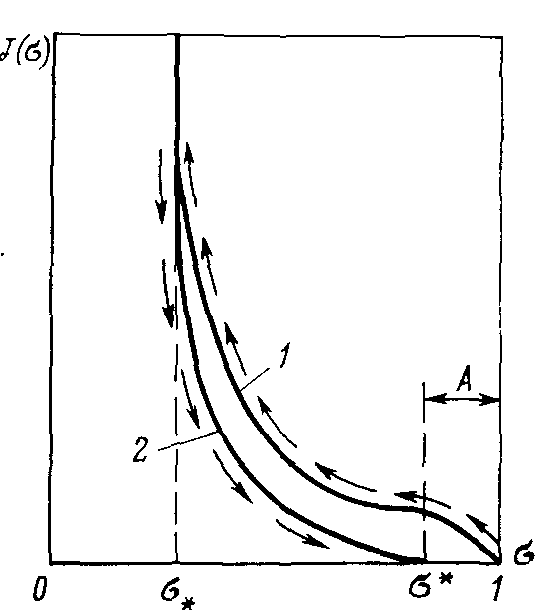
\includegraphics[width=.55\linewidth]{figures/fig-9-1.png}\caption{Зависимость капиллярного давления от насыщенности: \textit{1} --- кривая вытеснения; \textit{2} --- кривая пропитки; $A$ --- остаточная насыщенность вытесняемой жидкостью}\label{q10:fig-9-1}\end{figure}
Процессы многофазной фильтрации идут по-разному в зависимости от характерного времени фильтрационного процесса и от размеров области течения. Капиллярные силы создают в пористой среде перепад давления, величина которого ограничена и не зависит от размеров области фильтрации. Вместе с тем перепад внешнего давления, создающего фильтрационный поток между двумя точками, пропорционален скорости фильтрации и расстоянию между этими точками. Если размеры области малы, то при достаточно малых скоростях фильтрации капиллярные силы могут превзойти внешний перепад давления. Напротив, если рассматривается движение в очень большой области (например, в целой нефтяной или
% Источник: Basniev-et-al.djvu; печатная страница: 202; страница файла: 203
газовой залежи), то влияние капиллярных сил на распределение давления незначительно и их действие проявляется в локальных процессах перераспределения фаз. Взаимное торможение фаз, благодаря которому относительные фазовые проницаемости не равны соответствующим насыщенностям, обусловлено, прежде всего, капиллярными эффектами. В тех случаях, когда можно пренебречь капиллярным скачком $p_\text{к}(\sigma)$, капиллярность косвенно учитывается самим видом опытных кривых относительных проницаемостей $k_i(\sigma)$.

Таким образом, при описании многофазной фильтрации увеличивается число параметров, подлежащих определению. Наряду с неизвестными давлениями $p_i$ в фазах и скоростями фильтрации фаз $\vec w_i$ появляются новые неизвестные --- насыщенности $\sigma_i$ и концентрации отдельных компонентов. Это усложняет теоретическое исследование.

\subsection*{§ 3. Исходные уравнения многофазной фильтрации}
Будем для простоты рассматривать совместное изотермическое течение двух фаз в однородной пористой среде без фазовых переходов и химических реакций. Система уравнений, описывающая совместную фильтрацию фаз, строится на основе уравнений неразрывности для каждой фазы, уравнений движения (закона фильтрации) и соответствующих замыкающих соотношений.

\topic{Уравнения неразрывности}
Для вывода уравнения неразрывности рассмотрим баланс вытесняющей однородной жидкости (см. гл. 3). Выделим в фильтрационном потоке элементарный объем $\Delta V$ в форме прямоугольного параллелепипеда; $\Delta V=\Delta x\Delta y\Delta z$ (рис. \ref{q10:fig-9-2}). Площади его граней, параллельные координатным осям, соответственно равны: $\Delta\omega_x=\Delta y\Delta z$; $\Delta\omega_y=\Delta x\Delta z$; $\Delta\omega_z=\Delta x\Delta y$. Пусть $\vec q_1(x,y,z,t)=\rho_1\vec w_1$ --- вектор массовой скорости фильтрации первой фазы.
\begin{figure}[H]\centering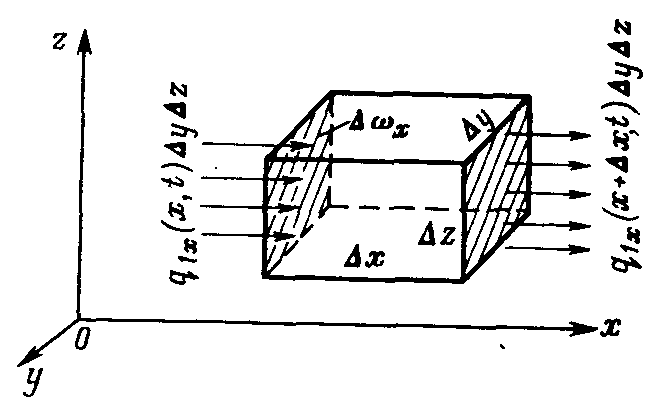
\includegraphics[width=.55\linewidth]{figures/fig-9-2.png}\caption{Схема к выводу уравнения неразрывности для $i$-й фазы}\label{q10:fig-9-2}\end{figure}
Для сжимаемой фазы ее плотность, масса и насыщенность в рассматриваемом элементарном объеме могут изменяться во времени. Если за некоторый промежуток времени в объем втекает большее количество жидкости, чем вытекает, то ее плотность и насыщенность в этом объеме увеличатся (и наоборот). Исходя из этих соображений, и сформулируем закон сохранения массы. Запишем баланс массы в направлении оси $Ox$. Через левую грань параллелепипеда (см. рис. \ref{q10:fig-9-2}) за промежуток времени $\Delta t$ втекает масса первой фазы, равная
% Источник: Basniev-et-al.djvu; печатная страница: 203; страница файла: 204
\[M_x^+=q_{1x}(x,y,z,t)\Delta y\Delta z\Delta t,\]
а через правую грань вытекает масса этой фазы, составляющая
\[M_x^-=q_{1x}(x+\Delta x,y,z,t)\Delta y\Delta z\Delta t.\]
Следовательно, прирост массы фазы в данном элементе объема, вызванный течением через эти две грани, равен $M_x^+-M_x^-$. Аналогично подсчитывается прирост массы и для других пар граней (соответственно в направлении осей $Oy$ и $Oz$). Тогда общее изменение массы в рассматриваемом объеме $\Delta V$ за время $\Delta t$ равно:
\begin{equation}\begin{aligned}
M^+-M^-={}&\{[q_{1x}(x,y,z,t)-q_{1x}(x+\Delta x,y,z,t)]\Delta y\Delta z+\\
&+[q_{1y}(x,y,z,t)-q_{1y}(x,y+\Delta y,z,t)]\Delta z\Delta x+\\
&+[q_{1z}(x,y,z,t)-q_{1z}(x,y,z+\Delta z,t)]\cdot\Delta x\Delta y\}\Delta t.
\end{aligned}\tag{9.7}\label{q10:eq-9-7}\end{equation}
С другой стороны, это изменение массы должно быть сбалансировано за счет изменения насыщенности и плотности массы фазы, находящейся внутри элементарного порового объема
\begin{equation}\Delta M=\left(\left.m\sigma\rho_1\right|_{x,y,z,t+\Delta t}-\left.m\sigma\rho_1\right|_{x,y,z,t}\right)\Delta x\Delta y\Delta z,\tag{9.8}\label{q10:eq-9-8}\end{equation}
где $m$ --- пористость среды, которая, вообще говоря, может меняться со временем.

Приравняв выражения \eqref{q10:eq-9-7} и \eqref{q10:eq-9-8}, разделив обе части полученного равенства на $\Delta x\Delta y\Delta z\Delta t$ и перейдя к пределу при $\Delta x,\Delta y,\Delta z$ и $\Delta t$, стремящихся к нулю, получаем
\[\frac{\partial q_{1x}}{\partial x}+\frac{\partial q_{1y}}{\partial y}+\frac{\partial q_{1z}}{\partial z}=-\frac{\partial(m\rho_1\sigma)}{\partial t},\]
откуда, заменяя $\vec q_1$ на $\rho_1\vec w_1$, окончательно находим
\[\frac{\partial(\rho_1w_{1x})}{\partial x}+\frac{\partial(\rho_1w_{1y})}{\partial y}+\frac{\partial(\rho_1w_{1z})}{\partial z}=-\frac{\partial(m\rho_1\sigma)}{\partial t},\]
или в векторной форме
\begin{equation}\frac{\partial}{\partial t}(m\rho_1\sigma)+\Div(\rho_1\vec w_1)=0.\tag{9.9}\label{q10:eq-9-9}\end{equation}
Аналогично выводится уравнение сохранения массы для второй фазы:
\begin{equation}\frac{\partial}{\partial t}[m\rho_2(1-\sigma)]+\Div(\rho_2\vec w_2)=0.\tag{9.10}\label{q10:eq-9-10}\end{equation}
Если вытесняемая и вытесняющая фазы --- слабосжимаемые упругие жидкости, то влиянием сжимаемости на распределение насыщенности можно пренебречь, так как время перераспределения давления за счет сжимаемости жидкостей, по крайней мере, на два порядка меньше, чем время вытеснения. Отсюда следует, что нестационарные процессы упругого перераспределения давления
% Источник: Basniev-et-al.djvu; печатная страница: 204; страница файла: 205
заканчиваются в начале процесса вытеснения. В некоторых случаях можно считать несжимаемым и газ в пластовых условиях.

Если жидкости и пористую среду можно предполагать несжимаемыми, то вместо уравнений \eqref{q10:eq-9-9} и \eqref{q10:eq-9-10} имеем
\begin{equation}m\frac{\partial\sigma}{\partial t}+\Div\vec w_1=0,\qquad-m\frac{\partial\sigma}{\partial t}+\Div\vec w_2=0.\tag{9.11}\label{q10:eq-9-11}\end{equation}
\topic{Уравнения движения для многофазной фильтрации}
При записи закона фильтрации будем предполагать, что в любой точке каждая из фаз находится в термодинамически равновесном состоянии. Тогда для течения двухфазной смеси можно ввести в рассмотрение относительные проницаемости $k_i(\sigma)$ и капиллярное давление $\rho_\text{к}(\sigma)$, зависящее только от насыщенности.
% В оригинале в этой фразе напечатано ρ_к, а в формулах p_к; сохранено.
Будем рассматривать только однонаправленные процессы фильтрации, не учитывая гистерезисных явлений.

Тогда выполняется закон фильтрации \eqref{q10:eq-9-4}:
\begin{equation}\vec w_i=-\frac{k}{\mu_i}k_i(\sigma)(\grad p_i-\rho_i\vec g),\tag{9.12}\label{q10:eq-9-12}\end{equation}
а связь между давлениями в фазах определяется равенствами \eqref{q10:eq-9-5} и \eqref{q10:eq-9-6}:
\begin{equation}p_2-p_1=p_\text{к}(\sigma)=\alpha_\text{п}\cos\theta\sqrt{\frac{m}{k}}J(\sigma).\tag{9.13}\label{q10:eq-9-13}\end{equation}
Для замыкания полученной системы уравнений необходимо задать связи параметров, характеризующих свойства фаз и пористой среды, с давлением.

\topic{Уравнения состояния флюидов}
При изотермических условиях фильтрации плотность и вязкость каждой из фаз определяются давлением в данной фазе:
\begin{equation}\rho_i=\rho_i(p_i),\qquad\mu_i=\mu_i(p_i),\qquad(i=1,2).\tag{9.14}\label{q10:eq-9-14}\end{equation}
Пласт будем считать недеформируемым.

Таким образом, получена замкнутая система уравнений \eqref{q10:eq-9-9}, \eqref{q10:eq-9-10}, \eqref{q10:eq-9-12}, \eqref{q10:eq-9-13} и \eqref{q10:eq-9-14} для определения всех неизвестных параметров: насыщенности $\sigma$, давления $p_i$, скорости фильтрации $\vec w_i$, плотности $\rho_i$ и вязкости $\mu_i$ фаз.

Постановка и решение задач на основе полной системы уравнений фильтрации неоднородных жидкостей затруднительны ввиду сложности самих уравнений, а также формулировки краевых условий, в частности разрыва капиллярных сил на границах пористой среды (так называемых «концевых эффектов»), роль которых недостаточно изучена.

Анализ одномерных двухфазных потоков позволяет выявить основные эффекты и характерные особенности совместной фильтрации жидкостей.

\end{document}
